\chapter{Arquitecturas para el cómputo de la Transformada Rápida de Fourier} \label{sec:cap_arqs}

En el capítulo anterior fue expuesta la utilidad de la iDFT y la DFT para la mdulación y
demodulación de señales en un sistema OFDM y las ventajas de los algoritmos FFT para el cálculo de
la transformada discreta de Fourier.

Siguiendo la terminología introducida por Burrus \cite{Burrus} \cite{Meyer3_1} se define como
\textit{algoritmos FFT} a aquellos donde se realiza un mapeo multidimensional de los índices en sus
entradas y salidas, como se explicó en la sección \ref{sec:fft}, dejando el término \textit{algoritmo DFT}
a aquellos algoritmos donde no se utiliza un mapeo multidimensional de los índices.

\section{Algoritmos DFT}

Los algoritmos DFT implementan el cálculo de la DFT aplicando optimizaciones sobre la
ecuación de síntesis.

\subsection{Algoritmo de Goertzel}

Cada componente del espectro de una señal $x_{[n]}$ en un cómputo de DFT puede escribirse como

\begin{equation}
	X[k] = x[0] + x[1]W_{N}^{k} + x[2]W_{N}^{2k} + \ldots + x[N-1]W_{N}^{(N-1)k}  
\label{eq:goertz1}
\end{equation}

Se pueden combinar todos los $x[n]$ con el mismo factor común $W_N^k$ obteniendo

\begin{equation}
	X[k] = x[0] + W_{N}^{k}(x[1] + W_{N}^{k}(x[2] + \ldots + x[N-1]W_{N}^{k} \ldots ))  
\label{eq:goertz2}
\end{equation}

Esta ecuación resulta en una posible implementación recursiva para el cálculo de $X[k]$. Este
cómputo es conocido como el algoritmo de Goertzel. Su mayor utilidad se encuentra para calcular un
número reducido de componentes espectrales ya que para el cálculo de una DFT completa la complejidad
llega a $\Theta(N^2)$, donde no representa ninguna mejora respecto al cálculo directo de la DFT
\cite{meyer_Goerts}.

\subsection{Transformación Bluestein Chirp-z}

En la transformación Bluestein Chirp-z el exponente \textit{kn} en \ref{eq:DTF} es expandido
cuadráticamente a 

\begin{equation}
	kn = -(k-n)^2/2 + n^2/2 + k^2/2  
\label{eq:chirp1}
\end{equation}

El cómputo de la DFT se reduce entonces a

\begin{equation}
	X[k] = W_{N}^{k^2/2}\sum_{n=0}^{N-1}(x[n]W_{N}^{n^2/2})W_{N}^{-(k-n)^2/2}  
\label{eq:goertz2}
\end{equation}

Entonces el cálculo de la DFT mediante este algoritmo se reduce a tres pasos:

\newcommand{\Conv}{\mathop{\scalebox{1.5}{\raisebox{-0.2ex}{$\ast$}}}}

\begin{itemize}
  \item N multiplicaciones de $x[n]$ por $W_{N}^{n^2/2}$
  \item Convolución lineal de $x[n]W_{N}^{n^2/2} \Conv W_{N}^{n^2/2}$
  \item N multiplicaciones por $W_{N}^{k^2/2}$
\end{itemize}

Para una transformación completa se necesita una convolución de longitud N y 2N multiplicaciones
complejas. Una ventaja de este algoritmo es que puede utilizarse para cualquier valor de N, sin la
limitación de que N sea par o potencia de 2 o 4 \cite{meyer_CZT}.

\subsection{Algoritmo DFT de Winograd}

El algoritmo de Winograd transforma el cómputo de la DFT en una convolución cíclica y aplica el
algoritmo de convolución de Winograd \cite{WinoConv}. La longitud de la DFT queda
restringida a números primos o potencias de números primos.
La transformación de la DFT en una convolución se realiza mediante el método Rader \cite{Rader}, en
el que partiendo de la premisa que N es un número primo se puede hallar un elemento generador
$g$ que genere todos los elementos $n$ y $k$ \cite{gener}, a excepción del $0$,  de forma que

 \begin{equation}
	X[k] = \sum_{n=0}^{N-1}x[n]W_{N}^{nk} \qquad k,n \; \displaystyle\epsilon \;
	\mathbb{Z_N}
\label{eq:rader1}
\end{equation}

Reemplazando $n$ por $g^n \thinspace mod \thinspace N$ y $k$ por $g^k \thinspace mod \thinspace N$
se obtiene el siguiente mapeo de índices:

\begin{equation}
	X[g^k \thinspace mod \thinspace N] - x[0] = \sum_{n=0}^{N-2}x[g^n \thinspace mod \thinspace N]
	W_{N}^{g^{n+k} \thinspace mod \thinspace N}
\label{eq:rader2}
\end{equation}

para $k \epsilon \{1,2,3 \ldots N-1\}$. Se puede notar que el lado derecho de \ref{eq:rader2} es una
convolución cíclica, i.e.,

\begin{equation}
	[x[g^0 \thinspace mod \thinspace N], x[g^1 \thinspace mod \thinspace N], \ldots, x[g^{N-2}
	\thinspace mod \thinspace N] \Conv [W_N, W_N^g, \ldots, W_N^{g^{N-2}
	\thinspace mod \thinspace N}]
\label{eq:rader2}
\end{equation}

Implementando la convolución con el algoritmo de Winograd se reduce la cantidad de multiplicaciones
no triviales aumentando así la eficiencia del cómputo de DFT \cite{WinoConv}.

\section{Álgoritmos FFT}

Los algoritmos FFT logran la eficiencia en el cómputo de la DFT a través de un mapeo
multidimencional de los coeficientes.

\subsection{Algoritmo de Cooley-Tuckey para el cálculo de FFT}

El algoritmo de Cooley-Tukey es el más universal de los algoritmos para cálculo
de FFT porque permite utilizar cualquier factorización de N \cite{Meyer2_2}. En particular
los algoritmos de Cooley-Tukey que transforman N en una potencia de base $r$,
$N=r^\nu$, son llamados \emph{Radix-r} y son los más populares \cite{Meyer2_2}.

La transformación de índices propuesta por Cooley y Tukey (y por Gauss
previamente) es también la más simple. Partiendo de
(\ref{eq:timeInedx}) y (\ref{eq:freqInedx}) se utilizan como coeficientes
$A=N_2$, $B=1$, $C=1$ y $D=N_1$ resultando en el mapeo:

\begin{equation}
n = N_2n_1 + n_2 \qquad 
	\begin{cases}
	0\leq n_1 \leq N_1 -1 \\
	0\leq n_2 \leq N_2 -1
	\end{cases}
\label{eq:CT_time_inedx}
\end{equation}

\begin{equation}
k = k_1 + N_1k_2 \qquad 
	\begin{cases}
	0\leq k_1 \leq N_1 -1 \\
	0\leq k_2 \leq N_2 -1
	\end{cases}
\label{eq:CT_freq_inedx}
\end{equation}

Dado el intervalo que pueden tomar $n_1$ y $n_2$ el cálculo del módulo no
necesita estar explícito.

Reemplazando $n$ y $k$ en $W_N^{nk}$ de acuerdo a (\ref{eq:CT_time_inedx}) y
(\ref{eq:CT_freq_inedx}):

\begin{equation}
W_N^{kn}=W_N^{N_2n_1k_1+N_1N_2n_1k_2+n_2k_1+N_1n_2k_2} 
\label{eq:Wkn}
\end{equation}

Como $W_N^{nk}$ es de orden $N=N_1N_2$ se llega a que $W_N^{N_1}=W_{N_2}$ y
$W_N^{N_2}=W_{N_1}$ que aplicado en \ref{eq:Wkn}:

\begin{equation}
W_N^{kn}=W_{N_1}^{n_1k_1}W_N^{n_2k_1}W_{N_2}^{n_2k_2} 
\label{eq:Wkn_red}
\end{equation}

Reemplazando (\ref{eq:Wkn_red}) en (\ref{eq:DTF}) se llega a:

\begin{equation}
X[k1,k2]=\sum_{n_2=0}^{N_2-1}
W_{N_2}^{n_2k_2}\left(W_{N}^{n_2k_1}\sum_{n_1=0}^{N_1-1}x[n_1,n_2]W_{N_1}^{n_1k_1}\right)
\label{eq:DFT_mod}
\end{equation}

La sumatoria interior en (\ref{eq:DFT_mod}) es una DFT de $N_1$ puntos que está
multiplicada por el factor $W_{N}^{n_2k_1}$. Definiendo
$\tilde{x}[n2,k1]=W_{N}^{n_2k_1}\sum_{n_1=0}^{N_1-1}x[n_1,n_2]W_{N_1}^{n_1k_1}$
y reemplazando en (\ref{eq:DFT_mod}) se llega a:

\begin{equation}
X[k1,k2]=\sum_{n_2=0}^{N_2-1}
W_{N_2}^{n_2k_2}\tilde{x}[n2,k1]
\label{eq:DFT_tilde}
\end{equation}

(\ref{eq:DFT_tilde}) muestra la DFT de $N_2$ puntos de $\tilde{x}$, lo que
representa la característica principal de este algoritmo, para cualquier valor de $N_1$ y $N_2$ tales que $N=N_1N_2$ la
DFT de longitud N de $x(n)$ se puede calcular siguiendo los siguientes pasos:

\begin{itemize}
  \item Transformar los índices de la secuencia de entrada según
  (\ref{eq:CT_time_inedx})
  \item Calcular la DFT de $N_1$ puntos de la secuencia $x(n)$.
  \item Multiplicar los puntos resultantes del paso anterior por el twiddle
  factor correspondiente.
  \item Calcular la DFT de longitud $N_2$ de la secuencia resultante del paso
  anterior.
  \item Transformar los índices de la secuencia de salida según
  (\ref{eq:CT_freq_inedx})
\end{itemize}

Nada impide aquí subdividir cualquiera de las DFT de la ecuación
(\ref{eq:DFT_tilde}) en dos DFT de longitudes menores sucesivamente hasta
obtener DFT de longitudes convenientes para realizar los cálculos.

Una ventaja del algoritmo de Cooley-Tuckey es la posibilidad del alojamiento en memoria
\textit{in-place} en el cual los resultados del cálculo de una etapa se guarda en memoria en las
mismas pocisiones que los valores utilizados para el cálculo, utilizando en forma eficiente la
memoria ya que para el cálculo de una DFT de $N$ puntos solo se requiere una memoria de longitud
$N$.

\subsubsection{Algoritmos radix-r}

Aprovechando la posibilidad que brinda el algoritmo de Cooley-Tuckey de poder factorizar $N$
libremente se puede optar por una factorización del tipo $N=r^\nu$. A los algoritmos de
Cooley-Tuckey de este estilo se los conoce como algoritmos \textit{radix-r}.
De esta manera el cálculo de la DFT se descompone en $\nu$ DFTs consecutivas de $r$ puntos cada una.

Por ejemplo para $r=2$ y $\nu$ etapas, $N=2^\nu$, el mapeo de índices queda como

\begin{equation}
n = 2^{\nu-1}n_{1}+\ldots+2n_{\nu-1}+n_{\nu}
\label{eq:radix2_n}
\end{equation}

\begin{equation}
k = k_1 + 2k_2+\ldots+2^{\nu-1}k_{\nu}
\label{eq:radix2_k}
\end{equation}

El número total de twiddle factors para un algortimo radix-2 es:

\begin{equation}
log_2(N)N/2
\label{eq:twf_radix2}
\end{equation}

La ventaja de esto es poder reducir el cálculo de  una DFT a múltiples cálculos de DFTs de tamaño
más pequeño y de cálculo más simple. Teniendo en cuenta por ejemplo que en el cómputo de una DFT de
longitud $2$ o $4$ no es necesario realizar ninguna multiplicación no trivial a excepción del
producto por el twiddle factor, eligiendo $N$ como potencia de $2$ o $4$ se reduce la cantidad de
multiplicaciones a realizar aumentando así la eficiencia del algoritmo.
 
\subsection{Algoritmo de Good-Thomas}

La transformación de índices sugerida por Good y Thomas transforma una DFT de longitud $N=N_1*N_2$
en una DFT bidimencional sin \textit{twiddle factors}, como si hay en el algoritmo de Cooley-Tukey.
El costo de la ausencia de \textit{twiddle factors} es la necesidad de que los factores $N_1$ y
$N_2$ deben ser coprimos (i.e., $gcd(N_k,N_l) = 1$ para $k \neq l$) y el mapeo se torna más
complicado al tener que realizar el cálculo de los índices en el momento y no poder utilizar tablas
precalculadas para ello.
Si se intenta eliminar los \textit{twiddle factors} introducidos por el mapeo de índices, según
\ref{eq:timeInedx} y \ref{eq:freqInedx}, se obtiene:

\begin{equation}
%	\begin{tabular}{r@{=}l}
	W_N^{nk} = W_N^{(An_1+Bn_2)(Ck_1+Dk_2)} \\
	         = W_N^{ACn_1k_1+ADn_1k_2+BCn_2k_1+BDn_2k_2}
%	\end{tabular}
\label{eq:GT_FFT}
\end{equation}

de donde surgen las siguientes condiciones necesarias que deben ser satisfechas en forma simultánea:

\begin{equation}
\langle AD \rangle_N = \langle BC \rangle_N = 0 
\label{eq:GT_cond1}
\end{equation}

\begin{equation}
\langle AC \rangle_N = N_2 
\label{eq:GT_cond2}
\end{equation}

\begin{equation}
\langle BD \rangle_N = N_1 
\label{eq:GT_cond3}
\end{equation}

El mapeo sugerido por Good y Thomas cumple con estas condiciones y está dado como sigue:

\begin{equation}
A=N_2 \qquad B=N_1 \qquad C=N_2 \langle N_2^{-1} \rangle_{N_1} \qquad D=N_1 \langle N_1^{-1}
\rangle_{N_2}
\label{eq:GT_mapping}
\end{equation}

Entonces

\begin{equation}
n = N_2n_1 + N_1n_2 \thinspace mod \thinspace N \qquad 
	\begin{cases}
	0\leq n_1 \leq N_1 -1 \\
	0\leq n_2 \leq N_2 -1
	\end{cases}
\label{eq:GT_time_inedx}
\end{equation}

\begin{equation}
k = N_2 \langle N_2^{-1} \rangle_{N_1}k_1 + N_1 \langle N_1^{-1}
\rangle_{N_2}k_2 \thinspace mod \thinspace N \qquad 
	\begin{cases}
	0\leq k_1 \leq N_1 -1 \\
	0\leq k_2 \leq N_2 -1
	\end{cases}
\label{eq:GT_time_inedx}
\end{equation}

Sustituyendo el mapeo de índices de Good-Thomas en la ecuación de la DFT (\ref{eq:DTF}) se obtiene

\begin{equation}
X[k1,k2]=\sum_{n_2=0}^{N_2-1}
W_{N_2}^{n_2k_2}\left(\sum_{n_1=0}^{N_1-1}x[n_1,n_2]W_{N_1}^{n_1k_1}\right)
\label{eq:GT_FFT_mod}
\end{equation}

La sumatoria interior en (\ref{eq:GT_FFT_mod}) es una DFT de longitud $N_1$. Definiendo
$\tilde{x}[n2,k1]=\sum_{n_1=0}^{N_1-1}x[n_1,n_2]W_{N_1}^{n_1k_1}$
y reemplazando en (\ref{eq:GT_FFT_mod}) se llega a:

\begin{equation}
X[k1,k2]=\sum_{n_2=0}^{N_2-1}
W_{N_2}^{n_2k_2}\tilde{x}[n2,k1]
\label{eq:GT_DFT_tilde}
\end{equation}

En este caso el procedimiento para el cómputo de la DFT mediante este algoritmo es similar al
procedimiento del algoritmo de Cooley-Tuckey pero sin la multiplicación intermedia por el
\textit{twiddle-factor}.

Existe una versión de este agoritmo conocido como el Algoritmo FFT de Winograd donde se
utiliza el mismo mapeo de Good-Thomas pero la DFT bidimensional resultante se resuelve utilizando el producto
de \textit{Kronecker} \cite{Meyer_Kron}.

\section{Selección del algoritmo}

\subsection{Algoritmos DFT y FFT} \label{sec:dftOfft}

Una métrica habitual a la hora de comparar los algoritmos de cómputo de DFT suele ser la cantidad de
multiplicaciones que deben realizarse, parámetro en que el algoritmo FFT de Winograd tiene el mejor
desempeño \cite{Meyer_Kron}, pero, dado que el dispositivo donde se va a implementar el algoritmo
puede tener unidades de cálculo de productos o similares, no debe ser este el único aspecto a tener
en cuenta.
La primera desición que debe tomarse es que tipo de algoritmo se utilizará, DFT o FFT. Para este
trabajo de tesis se seleccionará un algoritmo FFT ya que el mapeo multidimencional de los índices
permite dividir el cómputo de la DFT en cómputos más pequeños reduciendo la complejidad de la
implementación y permitiendo el uso de \textit{pipelines}\footnote{\label{pipeline} El pipelining
consiste en la división de un módulo combinacional en submódulos combinacionales entre los cuales
se colocan registros de modo de dividir la ejecución de todo el bloque en varios ciclos de clock,
lo que permite aumentar su frecuencia de trabajo} entre cada etapa de cómputo aumentando la
velocidad de procesamiento.

En la Tabla \ref{table:fft_comp}  se muestra una comparativa entre los distintos algoritmos FFT que
será tomada en cuenta para seleccionar cual será el algoritmo a implementar.

\begin{table}[h]
\begin{tabular}{l c c c}
\textbf{Propiedad} & \textbf{Cooley-Tuckey} & \textbf{Good-Thomas} & \textbf{Winograd} \\ \hline
Restricción sobre N & No & \multicolumn{2}{c}{Si. $gcd(N_k,N_l)=1$}\\ \hline
Máximo orden de $W$ & N & \multicolumn{2}{c}{$max(N_k)$} \\ \hline
Necesidad de \textit{Twiddle Factors} & Si & No & No \\ \hline
\# Multiplicaciones & bueno & bueno & mejor \\
\# Sumas & bueno & bueno & bueno \\
\# Esfuerzo de cómputo de índices & mejor & bueno & malo \\
\textit{Data in-place} & Si & Si & No \\ \hline
\end{tabular}
\caption{Comparativa entre algoritmos FFT}
\label{table:fft_comp}
\end{table}
 
Se puede apreciar en la tabla \ref{table:fft_comp} que el algoritmo de Cooley-Tuckey presenta las
mejores caraterísticas para uso general, siendo balanceada en cuanto a la cantidad de operaciones
aritméticas y la sobrecarga por el cómputo de los índices, pero ofreciendo la posibilidad de
utilizarla para cualquier valor de N.
Por este motivo se utilizará el algoritmo de Cooley-Tuckey para la implementación de este trabajo
de tesis, ya que la aplicación final de la arquitectura será como parte de un transmisor OFDM donde
no se puede limitar el número de puntos a las restricciones de los otros algoritmos mencionados. Además,
utilizando un algoritmo del tipo radix-r, se puede aprovechar la descompocisión en DFTs del mismo
tamaño reutilizando módulos tanto en la replicación de código como en un uso más eficiente de la
arquitectura una vez implementada.

\subsection{Arquitecturas radix-r}

Como se menciona en la sección \ref{sec:dftOfft} la arquitectura a implementar será de tipo radix-r.
En estos algoritmos se deben calcular $\nu$ DFTs de $r$ puntos cada una donde $N=r^\nu$. El valor
de $r$ toma importancia ya que la correcta elección del mismo puede conducir a implementaciones más
o menos eficientes. En la tabla \ref{table:fft_oper} se muestra la cantidad de operaciones
necesarias para bloques de DFT de distintos tamaños. Se considera como multiplicaciones triviales aquellas que son por $\pm 1$
y $\pm j$.

\begin{table}[h]
\begin{tabular}{c c c c}
\textbf{Long. del bloque} & \textbf{Multiplicaciones} & \textbf{Multiplicaciones no triviales} &
\textbf{sumas} \\ \hline 
$2$ & $2$ & $0$ & $2$ \\
$3$ & $3$ & $2$ & $6$ \\
$4$ & $4$ & $0$ & $8$ \\
$5$ & $6$ & $5$ & $17$ \\
$7$ & $9$ & $8$ & $36$ \\
$8$ & $8$ & $2$ & $26$ \\
$9$ & $11$ & $10$ & $44$ \\ \hline
\end{tabular}
\caption{Cantidad de operaciones complejas para distintas longitudes de DFT}
\label{table:fft_oper}
\end{table}

Se puede ver que para $r=2$ y $r=4$ no hay necesidad de realizar multiplicaciones no triviales
dentro de cada bloque DFT, quedando únicamente los productos por los twiddle factors. El siguiente
valor de $r$ en orden de eficiencia es $r=8$ que requiere dos multiplicaciones complejas por DFT.
Hay que tener en cuenta que si bien para un mismo valor de $N$ al aumentar el valor de $r$
disminuye la cantidad de etapas de DFT, también aumenta la complejidad de la implementación ya que
en cada bloque se deben procesar DFTs de $r$ puntos.
Teniendo en cuenta esto se decide implementar la arquitectura en dos versiones, utilizando $N=2$ y
$N=4$, ya que al ser valores pequeños permiten implementar la arquitectura para diversos valores de
$N$ manteniendo la complejidad de la implementación en niveles razonables, y se realizará un
análisis comparativo del rendimiento entre ellas.
Esto también implica que no es necesario agregar un multiplicador a los bloques DFT. Es por estos
motivos también que la mayoría de las implementaciones comerciales de bloques de cálculo de DFT se realizan con 
arquitecturas radix-2 y radix-4 \cite{radix_meyer}.

\subsubsection{Formas de implementar el algoritmo radix-r}\label{sec:radix}

En la figura \ref{fig:r2_8} se muestra un esquema simplificado de un algoritmo radix-2 de 8 puntos. 

\begin{figure}[htb!]
        \centering
        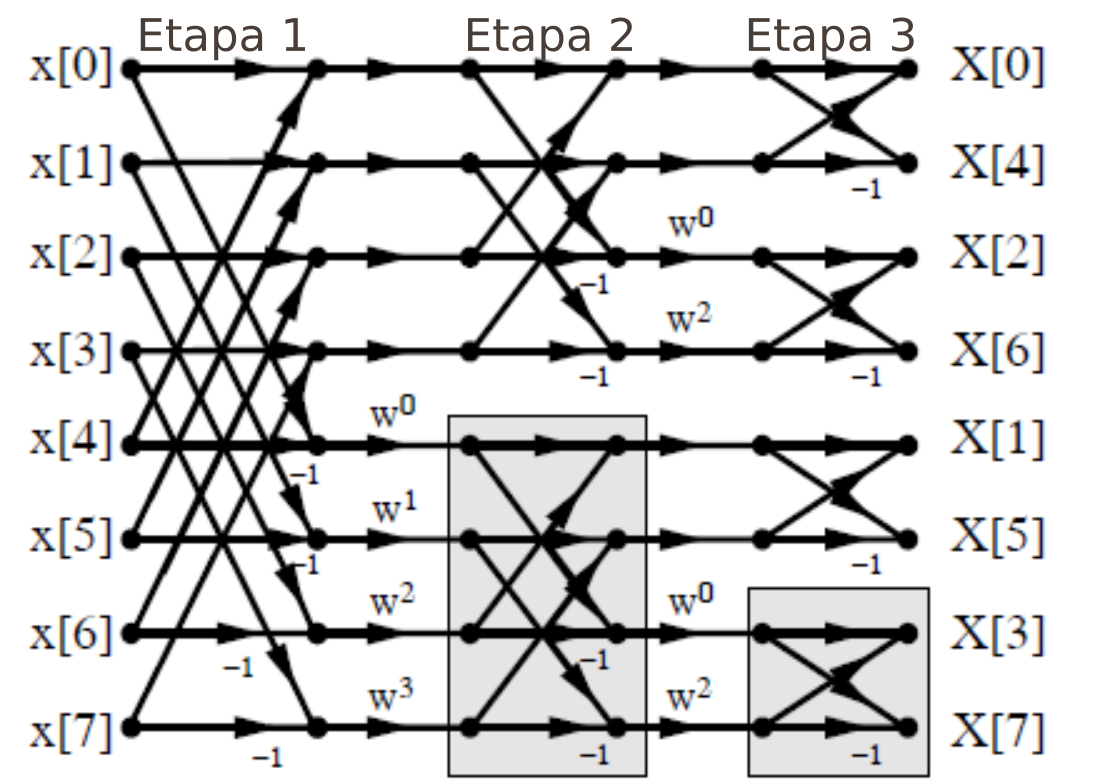
\includegraphics[width=10cm]{./figures/r2_8.png}
        \caption{FFT Radix-2 de 8 puntos}
        \label{fig:r2_8}
\end{figure}

En este esquema cada nodo donde llegan dos flechas representa una suma y cada flecha sobre una línea
representa un producto por el factor que la acompaña. Se aprecia claramente la división en etapas
en cada una de las cuales se realizan DFTs de $2$ puntos. Cada DFT de dos puntos es conocida como
\textit{butterfly} por la forma que toman las dos flechas cruzadas en el esquema de la figura
\ref{fig:r2_8}, en el caso de un algoritmo radix-4 el esquema es similar pero se realizan DFTs
tomando cuatro puntos. Se observa que para realizar una DFT de $8$ puntos se requieren $12$
\textit{butterflys}, generalizando $\frac{N}{2}*\log_2(N)$, y $8$ multiplicadores complejos,
generalizando $\frac{N}{2}*(\log_2(N)-1)$.
% Aquí se presentan variaciones en la forma en que se implementa el camino de
% los datos (\textit{datapath}) entre las distitintas etapas de cálculo de DFT. 
% La primer división surge en la cantidad de módulos DFT que se implementan. Las dos alternativas que
% surgen de esto son la implementación \textit{desenrollada} y la implementación \textit{iterativa}.
% 
% En la implementación desenrollada se utiliza un módulo de cómputo DFT (de $2$ o $4$ puntos según
% sea el caso) por etapa realizando de esta manera un cómputo DFT por etapa por ciclo de cálculo en
% paralelo, pasando los datos en serie de una etapa a la siguiente. La principal ventaja de esta
% implementación es que se tiene a la salida un punto por cada ciclo de cálculo. En la figura
% \ref{fig:r2sdf} se muestra un esquema de la arquitectura radix-2 SDF (Single-path Delay Feedback en
% inglés) \cite{torkelson} de 8 puntos donde se distinguen los bloques DFT de dos puntos y los
% multiplicadores para realizar el producto por el twiddle-factor. Se puede ver que la arquitectura
% consta de $log_2(8)=3$ etapas.
Existen diferentes variantes en la forma en que se implementa el camino de los datos
(\textit{datapath}), que implican diferencias en las cantidades de unidades de cómputo
\textit{butterfly} y de multiplicadores complejos. Las alternativas más comunes se listan a
continuación:

\begin{itemize}
  \item \textbf{Paralela} Se implementan todas las unidades \textit{butterfly} y multiplicadores
  complejos necesarios, dispuesto en una arquitectura similar al esquema de la figura
  \ref{fig:r2_8}. Se puede implementar en forma \textit{pipelined} colocando un banco de registros
  entre etapas concecutivas. La comunicación entre las etapas se realiza mediante un bus paralelo de
  tamaño $N$.
  \item \textbf{Desenrrollada} Arquitectura SDF (Single-path Delay Feedback en inglés)
  \cite{torkelson}. Se muestra un esquema de esta arquitectura para una FFT de $8$ puntos en la
  figura \ref{fig:r2sdf}. La comunicación se realiza mediante un bus serie, admitiendo un dato de
  entrada en cada ciclo de \textit{clock}. Se utiliza una unidad \textit{butterfly} por etapa,
  requiriendo en total $\log_\nu(N)$, y un multiplicador complejo por etapa excepto en la última
  dando un total de $ \log_\nu(N)-1$ multiplicadores. Se puede implementar en forma pipelined
  colocando un registro en medio de etapas concecutivas.
  \item \textbf{Iterativa} Se utiliza una única unidad \textit{butterfly} y un único multiplicador
  complejo para realizar secuencialmente las operaciones de todas las etapas. En la figura \ref{fig:r2sBf} se ve un esquema de la
  arquitectura radix-2 iterativa para $8$ puntos. 
\end{itemize}

\begin{figure}[htb!]
        \centering
        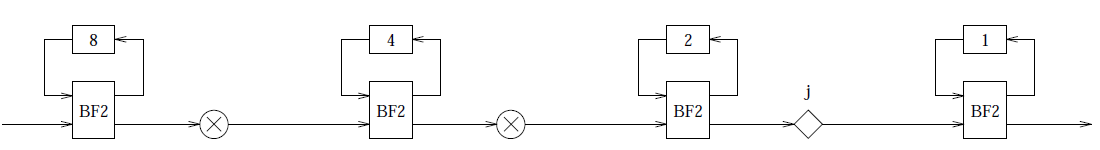
\includegraphics[width=13cm]{./figures/r2sdf.png}
        \caption{Arquitectura Radix-2 desenrollada SDF}
        \label{fig:r2sdf}
\end{figure}

% En la implementación iterativa se utiliza un único módulo de cómputo DFT con el que se calculan
% alternativamente cada una de las etapas, de a una por ciclo de cálculo. La principal ventaja de esta
% implementación es el menor tamaño respecto de la implementación desenrollada, lo que implica además
% menor consumo y una mayor eficiencia en la ocupación de los recursos. Por otro lado tiene como
% desventaja comparada con la versión desenrollada que ya no se tiene a la salida un punto nuevo por
% ciclo de cálculo sino que hay que esperar tantos ciclos de cálculo como etapas tenga la DFT a
% implementar, o sea, $\nu = log_r(N)$. En la figura \ref{fig:r2sBf} se ve un esquema de la
% arquitectura radix-2 iterativa para $8$ puntos. Aquí se realizan iterativamente todas las DFT de dos
% puntos con el mismo bloque ocupando un tercio del lugar que ocupa la arquitectura desentollada. En
% esta arquitectura se aprovecha el alojamiento en memoria in-place donde se reutiliza la pocisión de
% memoria ocupada por un punto luego de utilizarlo, para almacenar el valor resultante de ese cálculo.

\begin{figure}[htb!]
        \centering
        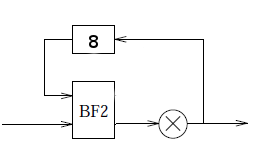
\includegraphics[width=6cm]{./figures/r2sBf.png}
        \caption{Arquitectura Radix-2 iterativa}
        \label{fig:r2sBf}
\end{figure}

En la tabla \ref{table:radixcomp} se realiza la comparativa entre las características distintivas de
cada implementación. El \textit{throughput} se toma como la cantidad y frecuencia con que se
obtienen puntos a la salida de la arquitectura. El campo \textit{pipelined} indica si la
implementación puede ser implementada de esa manera. En el caso del tamaño de memoria requerido no
se consideran implementaciones \textit{pipelined}, ya que en ese caso para la implementación
paralela hay que colocar N registros por cada etapa de \textit{ppipeline} que se coloca, mientras
que en la implementación desenrrollada se necesita un registro por etapa de \textit{pipeline}.

\begin{table}[htb!]
\centering
\begin{tabular}{l c c c}
\textbf{Característica} & \textbf{Radix paralela} & \textbf{Radix desenrrollada} &
\textbf{Radix iterativa}\\
\hline 
\# \textit{butterfly} & $\frac{N}{\nu}*\log_\nu(N)$ & $\log_\nu(N)$ & $1$ \\
\# multiplicadores & $\frac{N}{\nu}*(\log_\nu(N)-1)$ & $log_\nu(N)-1$ & $1$ \\
tamaño de memoria & $0$ & $N-1$ & $N$ \\
tipo de bus & Paralelo & Serie & Serie \\
\textit{throughput} & $N$ puntos por ciclo & $1$ punto por ciclo & $1$ punto cada $\log_\nu(N)$
ciclos\\
\textit{pipeline} & Si & Si & No\\
\hline
\end{tabular}
\caption{Comparativa entre las implementaciones paralela, desenrrolada e iterativa del algoritmo
radix-r}
\label{table:radixcomp}
\end{table}

Se puede observar que al aumentar el valor de $N$, la cantidad de puntos de la FFT a calcular,
aumenta la cantidad de unidades \textit{butterfly} y multiplciadores en las implementaciones
paralela, donde aumenta en forma proporcional, y en la desenrrollada, donde aumenta en forma
logarítmica, donde también aumenta el tamaño de la memoria. En la implementación iterativa un
aumento en la cantidad de puntos a procesar solo implica un aumento en memoria.

Teniendo en cuenta que el diseño de la arquitectura está orientado a su utilización en un sistema de
comunicación MIMO, no hay necesidad de un bus paralelo ya que los puntos de entrada llegan a la
arquitectura en serie, y son leídos de la misma manera, por el propio funcionamiento del sistema de
comunicación. En este sentido la implementación paralela queda prácticamente descartada. 
En cuanto al throughput, se puede operar la unidad de procesamiento FFT a una velocidad de
\textit{clock} mayor al resto del sistema para obtener el \textit{thoughput} necesario.

Se puede ver que la relación de tamaño entre la implementación desenrrollada y la iterativa
es del orden de $log_r(N):1$ para los módulos de cómputo aritmético. En base a la comparativa
realizada y al requerimiento de que la arquitectura sea económica en términos espaciales y de consumo se opta
por la implementación iterativa, ya que al aumentar $N$ solo se incrementa la cantidad de memoria
requerida manteniendo una arquitectura de tamaño reducido y bajo consumo. 

\subsection{Multiplicación por los twiddle factors} \label{sec:twiddlesec}

La implementación de multiplicadores en lógica digital es un tema delicado en cuanto al rendimiento
espacial y temporal. El cómputo de la DFT por el método de Cooley-Tuckey
requiere multiplicaciones complejas por los twiddle factors por lo que la forma de
implementar los multiplicadores no es un tema trivial. En una arquitectura desenrollada se necesitan
$log_r(N) - 1$ multiplicadores, dándole principal importancia al aspecto espacial de la
implementación, en tanto que en una arquitectura iterativa solo se necesita un único multiplicador
por lo que el aspecto principal a tener en cuenta es la velocidad de cómputo del multiplicador para
permitir una mayor frecuencia de cómputo.
Se analizan tres métodos para el cómputo del producto por los \textit{twiddle factors}.

\subsubsection{Algoritmo Cordic} \label{sec:cordicsec}

El producto por los twiddle factors, de la forma $W_N^{kn}=e^{\frac{-j2\pi kn}{N}}$, genera una
rotación en el plano complejo por lo que se puede reemplazar la multiplicación por una rotación.
En este sentido la primera opción que surge es la del algoritmo Cordic (Coordinate Rotation Digital
Computer sus siglas en inglés) que realiza rotaciones en dos dimenciones (además de otras
operaciones trigonométricas) en base únicamente a sumas/restas y desplazamientos.
Este algoritmo fue presentado en 1966 por Volder \cite{Volder} y es ampliamente utilizado para el
cálculo de funciones trigonométricas en sistemas digitales.

El principio de funcionamiento del algoritmo es realizar microrotaciones al vector inicial hasta
alcanzar una condición particular dependiente de una de las dos modalidades de funcionamiento: en
modo vectorial las coordenadas $(x_0,y_0)$ son rotadas hasta que $y_0$ converge a cero, en modo
rotacional el vector inicial $(x_0,y_0)$ es rotado un ángulo
$\theta_n$.
Esta rotación se lleva a cabo mediante microrotaciones por un ángulo $\theta_i$

\begin{equation}
x_{i+1} = x_i* \cos \theta_{i+1} - y_i* \sin \theta_{i+1}
\label{eq:micrototX}
\end{equation}

\begin{equation}
y_{i+1} = y_i* \cos \theta_{i+1} + x_i* \sin \theta_{i+1}
\label{eq:micrototY}
\end{equation}

Factorizando $\theta_{i+1}$ en (\ref{eq:micrototX}) y (\ref{eq:micrototY}) se obtiene:

\begin{equation}
x_{i+1} = \cos \theta_{i+1} (x_i - y_i* \tan \theta_{i+1})
\label{eq:micrototXfact}
\end{equation}

\begin{equation}
y_{i+1} = \cos \theta_{i+1} (y_i + x_i* \tan \theta_{i+1})
\label{eq:micrototYfact}
\end{equation}

Si se restringe $\tan \theta_{i+1}$ a $\pm 2^{-i}$ los productos del paréntesis pueden ser
reemplazados por desplazamientos aritméticos para cálculos en sistemas digitales de forma de
eliminar la necesidad de multiplicaciones en todas las iteraciones. El término $\cos \theta_{i+1}$
puede ser reemplazado por $\cos \theta_{i+1} = \cos (\arctan 2^{-i})$ definiendo las siguientes
variables:

\begin{equation}
K_i = \cos (\arctan 2^{-i}) = \frac{1}{\sqrt{1+2^{-2i}}}
\label{eq:micrototK}
\end{equation}

\begin{equation}
d_i = \pm 1
\label{eq:micrototd}
\end{equation}

Sabiendo que el coseno es una función impar, por lo que $\cos (\alpha) = \cos (-\alpha)$, y
reemplazando (\ref{eq:micrototK}) y /\ref{eq:micrototd}) en (\ref{eq:micrototXfact}) y
(\ref{eq:micrototYfact}) se obtienen las ecuaciones finales para el algoritmo Cordic:

\begin{equation}
x_{i+1} = K_i (x_i - y_i*d_i*2^{-i})
\label{eq:micrototXK}
\end{equation}

\begin{equation}
y_{i+1} = K_i (y_i + x_i*d_i*2^{-i})
\label{eq:micrototYK}
\end{equation}

La multiplicación por $K_i$ puede ser interpretada como una ganancia para todas las iteraciones por
lo que puede ser aplicada al final como una ganacia $K$ total del algoritmo igual a:

\begin{equation}
K = \prod K_i = \prod \frac{1}{\sqrt{1+2^{-2i}}}
\label{eq:Kprod}
\end{equation}

En cada iteración se debe decidir si $d_i = 1$ o $d_i = -1$, para lo cual se utiliza la diferencia
entre el ángulo deseado y el ángulo actual. Para ello se define una nueva variable como 

\begin{equation}
z_{i+1} = z_i - d_i \arctan 2^{-i}
\label{eq:zi}
\end{equation}

Y para decidir el valor de $d_i$ se utiliza

\begin{equation}
d_i =  
	\begin{cases}
	-1 \quad \sin z_i < 0 \\
	1 \quad \sin z_i \geq 0 
	\end{cases}
\label{eq:ni}
\end{equation}

$\arctan 2^{-i}$ puede ser calculado previamente y almacenado en tablas en memoria, al igual que el
valor de $K$, que al ser un valor definido para una cantidad determinada de iteraciones su
producto por el vector resultante puede ser calculado utilizando algoritmos eficientes para el
cómputo de productos.
En la figura \ref{fig:cordic} puede verse como se logra una rotación a través de microrotaciones a
lo largo de $4$ iteraciones.

\begin{figure}[htb!]
        \centering
        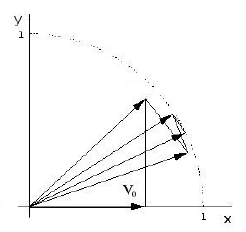
\includegraphics[width=6cm]{./figures/cordic.png}
        \caption{Ejemplo de rotación con algoritmo Cordic}
        \label{fig:cordic}
\end{figure}

Este algoritmo presenta como ventaja que solo utiliza sumas y desplazamientos para el cálculo de una
rotación vectorial, y la posibilidad de implementar las
etapas iterativas a través de un \textit{pipeline} para aumentar la frecuencia de trabajo. 

\subsubsection{Algoritmo BKM}

El algoritmo BKM busca, al igual que el algoritmo Cordic, resolver funciones elementales a través de
la utilización de sumas y desplazamiento de forma de poder implemetnarlas eficientemente en sistemas
digitales.
Este algoritmo se basa en las siguientes ecuaciones de recurrencia:

\begin{equation}
	\begin{cases}
	L_{n+1} = L_n(1+d_n*2^{-n}) \\
	E_{n+1} = E_n - \ln (1+d_n*2^{-n})
	\end{cases}
\label{eq:BKM}
\end{equation}

con $d_n \epsilon \{-1,0,1,-i,i,1-i,1+i,-1-i,-1+i\}$. 
Hay dos modos de operación del algoritmo. En el modo $L$ se itera hasta obtener $L_n=1$, entonces se
obtiene $E_n=E_1+\ln (L1)$. En el modo $E$ se itera hasta obtener $E_n=0$, entonces se obtiene
$L_n=L_1*\exp{E_1}$.
Es necesario precalcular y almacenar en memoria los valores de $\ln(1+d_n*2^{-n})$ para restárselo a
$E_1$ en cada iteración. La deducción y demostración del agoritmo es compleja y se puede ver en
\cite{BKM} así como ejemplos de aplicación para el cálculo de varias operaciones complejas y trigonométricas.
Para el cálculo del producto por los twiddle factors se utiliza la capacidad del algoritmo de
calcular la rotación de un vector $[a,b]$ por un ángulo $\theta$, utilizándo el modo $E$ con
$L1=a+ib$ y $E1=i\theta$.

Comparándolo con el algoritmo Cordic, ambos brindan la posibilidad de reducir el producto por los
twiddle factors a sumas y desplazamientos, con una complejidad espacial y computacional similar,
aunque el BKM requiere mayor almacenamiento en memoria que el Cordic. Los dos tienen la
característica de necesitar $p$ iteraciones para obtener $p$ bits de resolución. La principal
diferencia se da en la complejidad de implementación del algoritmo, donde el BKM es más complejo que
el Cordic, y en el hecho de que la principal ventaja del algoritmo BKM se da en implementaciones con
sistemas numéricos redundantes \cite{BKM}. Dado que la arquitectura a implementar en el presente
trabajo de tesis se hará utilizando el sistema numérico conocido como \textit{complemento a 2} (no
redundante) el algoritmo BKM no provee ninguna ventaja por sobre el algoritmo Cordic, siendo por el
contrario más complejo de implementar. Por este motivo de desestima su uso en este proyecto.

\subsubsection{Multiplicador complejo eficiente}

El uso extendido del algoritmo Cordic en arquitecturas de cómputo de FFT se justifica por el costo
espacial de implementar multiplicadores en sistemas digitales.
Pero dado que en este caso se necesita solo un multiplicador para toda la arquitectura, la
diferencia en el espacio requerido por el algoritmo Cordic y un multiplicador complejo no es
significativa (caso distinto para una implementación desenrollada donde se requieren $log_r(N)$
multiplicaciones).

En el caso del producto por los twiddle factors se requiere realizar una multiplicación compleja de
la forma:

\begin{equation}
R+jI = (A+jB)*(C+jD) = (A*C-B*D) + j(A*D+B*C)
\label{eq:prodcomp4}
\end{equation}

donde $(C+iD)$ es el twiddle factor. La implementación directa implica el uso de $4$
multiplicadores.
Se pueden precalcular y almacenar en una tabla determinados valores respecto a los twiddle factor
obteniendo una implementación más eficiente del producto complejo, como se explica a continuación.

Se precalculan y almacenan en memoria los valores $C$, $C+D$ y $(C-D)$. Con estos tres factores
precalculados se calcula:

\begin{equation}
\begin{split}
E &= A-B \\
Z &= C \times E = C \times (A-B)
\end{split}
\label{eq:prodcompZ}
\end{equation}

Y se computa el producto final como:

\begin{equation}
R = (C-D) \times B + Z
\label{eq:prodcompR}
\end{equation}

\begin{equation}
I = (C+D) \times A - Z
\label{eq:prodcompI}
\end{equation}

Como se indicó al principio de esta sección, al requerirse una única multiplicación compleja la
diferencia entre los costos espaciales de un multiplicador complejo y el algoritmo Cordic no es
significativa, por lo que se decide implementar el multiplicador complejo y evaluar su performance
respecto del algoritmo Cordic para decidir cual es mejor desde el punto de vista tanto de la
implementación como de la performance. Teniendo en cuenta que muchas FPGA cuentan con
unidades de procesamiento de señales, incluyendo multiplicadores, la implementación
de un multiplicador complejo tiene amplias ventajas sobre las demás opciones.

\subsection{Método de redondeo o truncamiento} \label{sec:redond}

El proceso de cómputo de la DFT mediante el método Radix requiere una serie
de sumas y restas, por lo que existe el riesgo de que se produzca desbordamiento (\textit{overflow}
en inglés) de la unidad aritmética. Para alamecenar el resultado de una suma entre dos operandos de $N$ bits
sin riesgo de desbordamiento se debe guardar el resultado en un número de $N+1$ bits. Esto
implicaría incrementar en $1$ el ancho de palabra de la aquitectura en cada etapa de cómputo.\\ 
Otra opción es la implmentación de un mecanismo de reducción del valor luego de una operación de suma y/o
resta dividiéndolo por $2$, ya que puede realizarse en forma trivial mediante un dezplazamiento
hacia la derecha. Debe tenerse en cuenta que este método introduce error en el resultado ya que la
dividir por $2$ se pierde información.\\
Se decide utilizar la segunda opción por su simplicidad de implementación y porque su tamaño no
depende de la cantidad de etapas a implementar. Para esto se evalua la implementación de un
mecanismo de redondeo y/o truncamiento para procesar el valor resultante de la división.

El redondeo y el truncamiento se utilizan para eliminar cifras no significativas en un número. En
este caso, su utilidad es la de eliminar el último bit del número que se divide por $2$ para
evitar el overflow.

El truncamiento consiste en eliminar las cifras no siginicativas descartándolas directamente.
El redondeo consiste en eliminar las cifras no significativas pero se suma $1$ al número resultante,
en caso que la última ciffra eliminada sea mayor o igual a la mitad de la base del sistema numérico, 
o no se suma nada en caso contrario.

En la Tabla \ref{table:redond} se muestran algunos ejemplos de la diferencia entre truncamiento y
redondeo al quitar el último digito decimal a cada número.

\begin{table}[htb!]
\centering
\begin{tabular}{c c c c}
\textbf{Número original} & \textbf{Truncamiento} & \textbf{Redondeo} \\ \hline 
$2.3641$ & $2.364$ & $2.364$ \\
$4.3156$ & $4.315$ & $4.316$ \\
$7.6355$ & $7.635$ & $7.636$ \\ \hline
\end{tabular}
\caption{Ejemplos de truncamiento y redondeo en sistema decimal}
\label{table:redond}
\end{table}

En el caso del redondeo en aritmética binaria, si el primer dígito eliminado es $1$ se le suma $1$
al número resultante y si es $0$ no se suma.

Se puede observar que el método de truncamiento introduce un error mayor al que introduce el método
de redondeo ya que el primero tiene una desviación máxima del valor real de una unidad mientras que
en el segundo la desviación máxima es de la mitad de una unidad.

Dado que la probabilidad de overflow depende de la magnitud de los puntos de entrada y que aplicar
cualquier de los dos métodos de aproximación introduce error se decide implementar un mecanismo de
división del resultado de la suma configurable en forma dinámica, en cuya configuración se puede
habilitar y deshabilitar la opción etapa por etapa y decidir si se aplica truncamiento o redondeo en
caso de habilitar la división.

\subsection{Arquitecturas a implementar}

De lo expuesto a lo largo del capítulo se decide implementar las siguientes arquitecturas:

\begin{itemize}
  \item Arquitectura radix-2 iterativa
  \item Arquitectura radix-4 iterativa
  \item Algoritmo cordic para el producto por los twiddle factor para las dos arquitecturas
  \item Multiplicador complejo para el producto por los twiddle factor para las dos arquitecturas
  como alternativa al algoritmo Cordic
  \item Mecanismo de división por dos a la salida del sumador/restador con posibilidad de
  seleccionar truncamiento o redondeo en forma dinámica.
\end{itemize}

La implementación de las arquitecturas se describe en el siguiente capítulo.
